%!TEX root = ./seminar.tex
\section{The Future of Digital Healthcare}
\subsection{Secure Management of Patient Data}
With the digitization of healthcare environments a lot of patient data must be stored and accessed by algorithms. While this in itself is of less concern, security measurements need to be taken to prevent unauthorized access to this data. In addition, countries like Germany take confidentiality and security of data seriously and therefore have very strict regulations regarding storage, usage and even collection of said data \cite{dsgvo}. Regardless of security concerns, the race for your data has already begun, with Apple releasing Apple Health Record and Apple Watch with a single-lead ECG \cite{appleHealth}. Joining Google with Google Fit and their WearOS - an operating system for smartwatches. Introducing Big Data concepts in the public healthcare sector may shift the focus from reactive to proactive care, reducing running costs and improving efficiency. This spans nearly all aspects of healthcare like diagnosis, treatment and population health management, to name a few. Furthermore, in moving from a volume-based to a value-based business model, healthcare providers see availability and accuracy of patients health data as pivotal. Now concerning security, healthcare data is stored in data centers with varying levels of security. They receive giant amounts of data from an even broader variety of sources. A first step to manage this data effectively and secure, is to introduce common data representations and local and regional standards. This allows the implementation of secure protocols for transportation and analysis in real-time. Currently, the healthcare industry is facing Distributed Denial of Service (DDoS) attacks, malware and social engineering attacks among others. As IoT environments are a big part of digital healthcare, their security is yet another problem, as implementing security in resource-constrained networks is an ever arising challenge. An approach would be to develop scaling key management solutions for secure transport of data in reasonable time-constraints. A last point that is key to patient privacy and data confidentiality is anonymization of data prior to anaytics \cite{patil2014big}.
\subsection{Artificial Intelligence in Healthcare}
Based on gathering and analyzing the vast amounts of data, powerful algorithms are now needed to ensure real-time and accurate usage to benefit patients in care. As the much praised (and feared) Artificial Intelligence (AI) expands its growth into the medical sector, patients already do, and further will, benefit from medical care that is tailored to their needs in a whole new way: proactively. Figure~\ref{fig:FDA_AI_Info} shows a timeline of Food and Drug Administration (FDA) approved AI-based algorithms in medicine since 2014 up until September 2019.
\begin{figure}[htp]
    \centering
    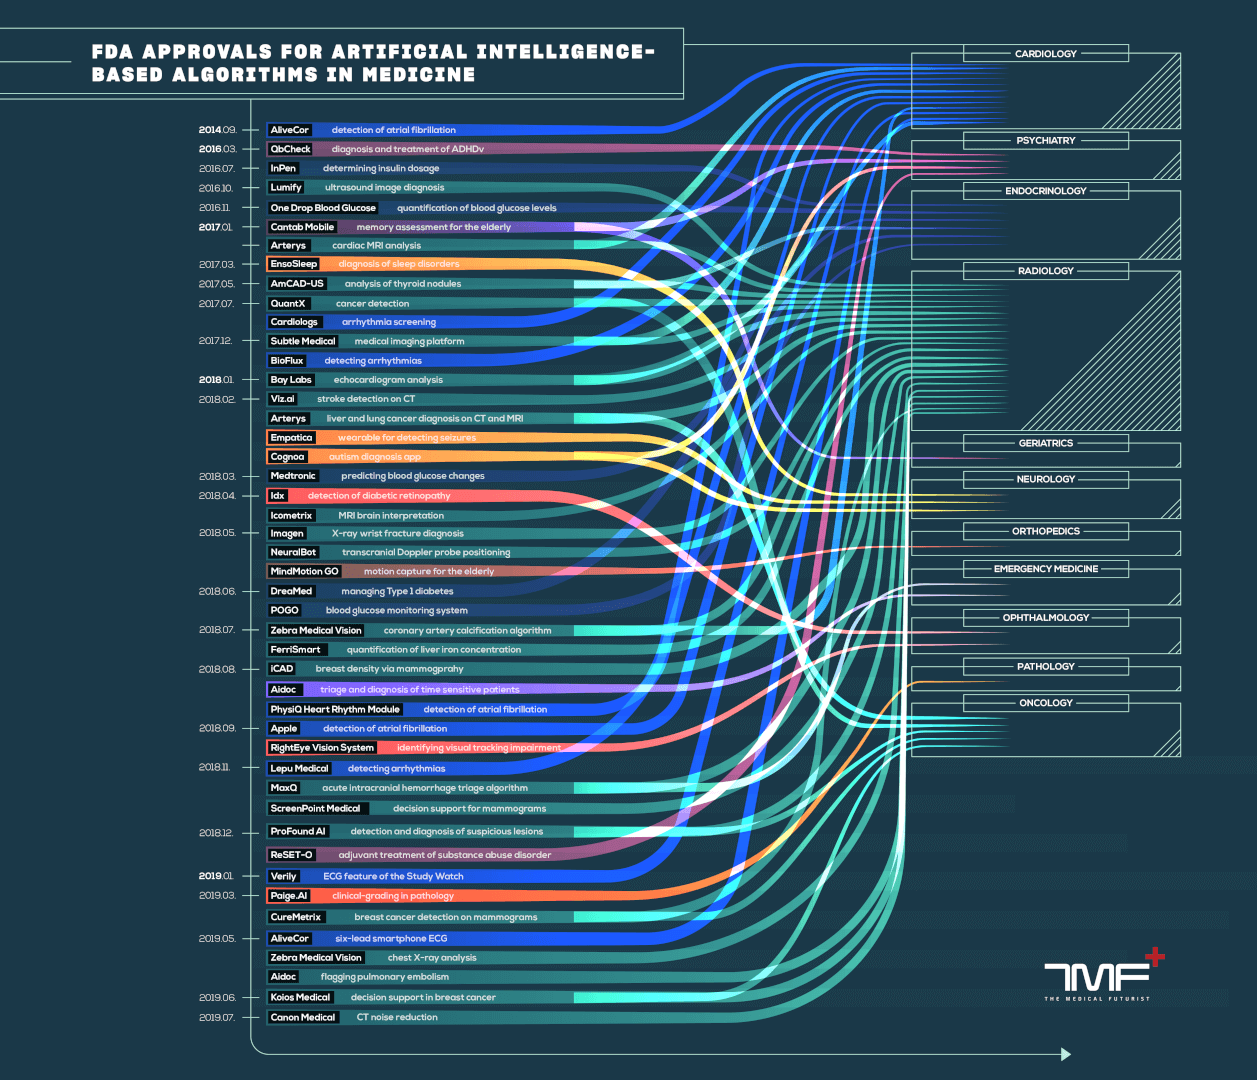
\includegraphics[width=\textwidth]{media/The-Medical-Futurist-FDA-approved-AI-algorithms-in-medicine-2019-09.png}
    \caption{FDA Approvals for Artificial Intelligence-Based Algorithms in Medicine - Infographic \cite{fdaAi}}%
    \label{fig:FDA_AI_Info}
\end{figure}
This looks very promising at least for the US healthcare environment. Meanwhile the current state in Germany is a bit less impressive. AI is used none the less, mostly for routine procedures and documentation, e.g. text assistance, error detection and detection of abnormalitites to prevent fraud. More diagnosis-based tasks include scanning unobtrusive x-ray images for cancer detection, giving doctors more time to look into more urgent cases. But while better image processing software enters the market, a low degree of digitization prevents them to work effectively, again highlighting the importance of a solid foundation in data collection and management \cite{kiKroenung}. A promising application of AI is developed in stroke detection and treatment. Stroke is the leading cause of death in China and the fifth in North America. 85\% of strokes are caused by cerebral infarction. As early symptoms often are not detected properly, only few patients receive timely treatment. The possible solution consists of two Machine Learning (ML) algorithms, namely genetic fuzzy finite state machine and PCA, that are used in a movement-detecting device for early stroke prediction \cite{villar2015improving}. Meanwhile the diagnosis of stroke relies on neuroimaging techniques like MRI and CT. Here, studies used ML methods to assist stroke diagnosis, reaching an accuracy of almost 90\% \cite{rehme2014identifying}.
\subsection{Individually Tailored Care}
Predictions regarding the future of the use of AI in medical environments suggest that it will be mostly patient-driven, meaning that patients will use and benefit from AI-based medical services outside of hospitals and doctors offices as they become increasingly commercialized and open to the public. This would accelerate the degree of customized care, as these personal devices have maximal information about their user while communicating his or her troubles to the data centers of healthcare providers to get feedback, similar cases and possible treatment \cite{kiKroenung}.
\subsection{Smart Implants}
While the previously mentioned wearable sensors can track a wide variety of health indicators, intrusive systems are on their way. Smart implants provide far more accurate stimuli and monitoring then vibration modules and sensors on the wrist can offer. Made from biocompatible material and equipped with low power microelectronics these devices can effectively transmit data from inside the body \cite{andreu2015wearable}. A prime example is an insulin implant that measures blood glucose levels in diabetics and releases insulin accordingly into the bloodstream \cite{rege2017development}. Another application is in surgery, monitoring white blood cells and neutrophil counts to prevent postoperative sepsis \cite{venema2013robustness}. Active and noninterruptible implants like pacemakers may be powered wireless by ultrasonic links doubling as a data communication path \cite{ozeri2010ultrasonic}.
\subsection{Value-Based Healthcare}

